\documentclass[24pt,a1paper,landscape,colspace=35pt]{tikzposter}
\usepackage{fontspec}
\setmainfont{Optima Medium.ttf}
% \usepackage[T1]{fontenc}
% \usepackage{tgpagella}

%═══════════════════════════════════════════
% Math packages
%═══════════════════════════════════════════
\usepackage{amssymb,amsthm,amsmath}
\usepackage{mathtools}
\usepackage{proof}
\usepackage{bussproofs}
\usepackage{marvosym}

%═══════════════════════════════════════════
% Environments
%═══════════════════════════════════════════
\theoremstyle{definition}
\newtheorem{definition}{Definition}
\newtheorem{theorem}{Theorem}
\newtheorem{lemma}[theorem]{Lemma}
\newtheorem{claim}{Claim}
\newtheorem{corollary}{Corollary}
\newtheorem{proposition}{Proposition}
\newtheorem{example}{Example}
\newtheorem{remark}[theorem]{Remark}
\newenvironment{sketch}{\begin{proof}[Proof Sketch]}{\end{proof}}

%═══════════════════════════════════════════
% Graphics packages
%═══════════════════════════════════════════
\usepackage{tikz}
\usepackage{graphicx}
\usetikzlibrary{positioning,calc,arrows.meta,shapes.geometric,fit, backgrounds}

% Colors
\definecolor{gruvwhite}{HTML}{fbf1c7}
\definecolor{gruvgreen}{HTML}{79740e}
\definecolor{gruvblue}{HTML}{076678}
\definecolor{gruvpurple}{HTML}{8f3f71}
\definecolor{gruvyellow}{HTML}{d79921} % b57614
\definecolor{gruvred}{HTML}{9d0006}
\definecolor{gruvblack}{HTML}{3c3836}
\definecolor{gruvgrey}{HTML}{ebdbb2} %7c6f64

% Colors
\colorlet{backgroundcolor}{gruvblack}
\colorlet{blockbodybgcolor}{gruvwhite}
\colorlet{blockbodyfgcolor}{black}
\colorlet{blocktitlefgcolor}{gruvwhite}
\colorlet{blocktitlebgcolor}{gruvred} % default, but changeable
\colorlet{framecolor}{gruvred}
\colorlet{titlefgcolor}{black}
\colorlet{titlebgcolor}{gruvwhite}


\colorlet{notebgcolor}{gruvblue}
\colorlet{notefgcolor}{gruvgreen}
\colorlet{noteframecolor}{gruvred}

%═══════════════════════════════════════════
% Custom Commands, General Use
%═══════════════════════════════════════════
\newcommand{\key}[1]{\emph{#1}}
\newcommand{\Rat}{\mathbb{Q}}
\newcommand{\Nat}{\mathbb{N}}
\newcommand{\State}{\mathsf{State}} 
\newcommand{\semantics}[1]{[\![\mbox{\em $ #1 $\/}]\!]}
\newcommand{\Model}{\mathcal{M}}
\newcommand{\Nodel}{\mathcal{N}}
\newcommand{\lang}{\mathcal{L}}
\newcommand{\uplang}{\mathcal{L}^\ast}
\newcommand{\vocab}{\mathcal{V}}
\newcommand{\wocab}{\mathcal{W}}
\newcommand{\set}[1]{\{ #1 \}}
\newcommand{\proves}{\vdash}
\renewcommand{\o}{\cdot}
\newcommand{\orr}{\vee}
\newcommand{\andd}{\wedge}
\newcommand{\nott}{\neg}
\newcommand{\bigandd}{\bigwedge}
\newcommand{\quadiff}{\quad \mbox{ iff } \quad}
\newcommand{\rem}[1]{\relax}
 \newcommand{\NP}{\mbox{\sc np}}
\newcommand{\axiom}{\textsc}
\newcommand*{\bigchi}{\mbox{\Large$\chi$}}% big chi
\newcommand{\degree}[1]{\mathrm{deg}(#1)}
\newcommand{\preds}[1]{\mbox{preds}(#1)}
\newcommand{\layer}[1]{\mathsf{layer}(#1)}
\newcommand{\activ}[2]{\mathsf{activ}_{#1}(#2)}
\newcommand{\layerNoArgs}{\mathsf{layer}}

\newcommand{\negweightscore}[1]{\mathsf{nws}(#1)}
\newcommand{\minscore}{\mathsf{mnws}}
\newcommand{\numiterations}{\mathsf{iter}}

%═══════════════════════════════════════════
% Custom Commands, Hebbian Learning
%═══════════════════════════════════════════
\newcommand{\AllNets}{\mathsf{Net}}
\newcommand{\Net}{\mathcal{N}}
\newcommand{\op}{\mathsf{op}}
\newcommand{\Prop}{\mathsf{Prop}}
\newcommand{\Reach}{\mathsf{Reach}}
\newcommand{\Hebb}[2]{\mathsf{Hebb}(#1, #2)}
\newcommand{\HebbNoArgs}{\mathsf{Hebb}}
\newcommand{\Hebbstar}[2]{\mathsf{Hebb}^*(#1, #2)}
\newcommand{\HebbstarNoArgs}{\mathsf{Hebb}^*}
\newcommand{\hebbweight}{W_\mathsf{Hebb}}
\newcommand{\hebbstarweight}{W_{\mathsf{Hebb}^*}}

\newcommand{\Typ}[1]{\textrm{\textup{\textbf{T}}} #1}
\newcommand{\Know}[1]{\textrm{\textup{\textbf{K}}} #1}
% \newcommand{\Know}[2]{\textrm{\textup{\textbf{K}}}(#1, #2)}
\newcommand{\KnowNoArgs}{\textrm{\textup{\textbf{K}}}}
\newcommand{\TypNoArgs}{\textrm{\textup{\textbf{T}}}}
% \newcommand{\Hebbop}[1]{[#1]_\textrm{\textup{hebb}\:}}
% \newcommand{\Hebbop}[1]{[#1]_{\HebbstarNoArgs}\:}
\newcommand{\Hebbop}[1]{[#1]}

\newcommand{\diaTyp}[1]{\langle \textrm{\textup{\textbf{T}}} \rangle #1}
\newcommand{\diaKnow}[1]{\langle \textrm{\textup{\textbf{K}}} \rangle #1}
% \newcommand{\diaKnow}[2]{\langle \textrm{\textup{\textbf{K}}} \rangle(#1, #2)}
\newcommand{\diaTypNoArgs}{\langle \textrm{\textup{\textbf{T}}} \rangle}
\newcommand{\diaKnowNoArgs}{\langle \textrm{\textup{\textbf{K}}} \rangle}
% \newcommand{\diaHebbop}[1]{\langle #1\rangle_\textrm{\textup{hebb}}}
\newcommand{\diaHebbop}[1]{\langle #1\rangle}

\settitle{ \centering \vbox{
\@titlegraphic \\[\TP@titlegraphictotitledistance] \centering
\color{titlefgcolor} {\bfseries \Huge \sc \@title \par}
\vspace*{0.5em}
{\Large \@author \par} \vspace*{0.5em} {\Large \@institute}
}}

\title{Reduction Axioms for Iterated Hebbian Learning}
\author{Caleb Schultz Kisby, Sa\'{u}l A. Blanco, Lawrence S. Moss}
\institute{Indiana University}



\begin{document}
\maketitle[roundedcorners=14,
titletotopverticalspace=20pt,
titletoblockverticalspace=40pt,
linewidth=7pt, 
innersep=20pt]

\begin{columns}
    \column{0.30}
    
    %======================================================
    % Block 1: Neural Network Semantics
    %======================================================
    \block[roundedcorners=14,linewidth=8pt]{Neural Network Semantics}{
        \begin{tikzfigure}%
            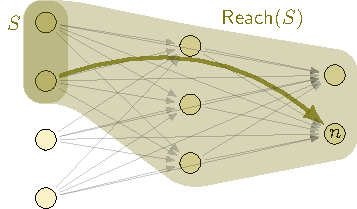
\includegraphics[width=0.8\linewidth]{figures/fig-reach.pdf}
        \end{tikzfigure}

        \begin{tikzfigure}%
            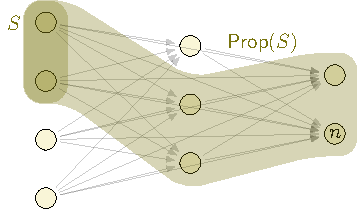
\includegraphics[width=0.8\linewidth]{figures/fig-prop.pdf}
        \end{tikzfigure}
    }
    
    %======================================================
    % Block 2: The Interpretation
    %======================================================
    \block[roundedcorners=14,linewidth=8pt]{The Interpretation}{
        
        \[
        \begin{array}{l}
        \mbox{Propositions are fixed sets of neurons}\\
        \begin{array}{lcl}
            \semantics{\neg \varphi} & = & \semantics{\varphi}^\complement \\
            \semantics{\varphi \land \psi} & = & \semantics{\varphi} \cap \semantics{\psi} \\
            \semantics{\diaKnow{\varphi}} & = & \Reach(\semantics{\varphi}) \\
            \semantics{\diaTyp{\varphi}} & = & \Prop(\semantics{\varphi})
        \end{array}
        \end{array}
        \]
    }

    \column{0.40}

    %======================================================
    % Block 3: Hebb*: Iterated Hebbian Learning
    %======================================================
    \block[roundedcorners=14,linewidth=8pt]{Iterated Hebbian Learning}{
        
        \begin{tikzfigure}%
            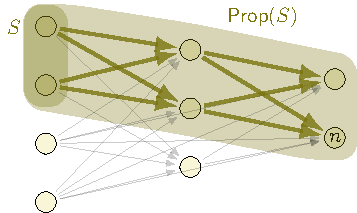
\includegraphics[width=0.56\linewidth]{figures/fig-hebb.pdf}
        \end{tikzfigure}
    }

    %======================================================
    % Block 4: The Reduction
    %======================================================
    \block[roundedcorners=14,linewidth=8pt]{The Reduction}{
        Our Main Result (highlight): Iterated Hebbian learning reduces to reasoning about forward Prop and graph Reach!

        \begin{theorem}
            The following axioms are sound.
            \[
            \begin{array}{lcll}
                \Hebbop{\varphi} p & \leftrightarrow & p \quad \quad \mbox{ for propositions } p \\
                \Hebbop{\varphi} \neg \psi & \leftrightarrow & \neg \Hebbop{\varphi} \psi\\
                \Hebbop{\varphi} (\psi \land \rho) & \leftrightarrow & \Hebbop{\varphi} \psi \land \Hebbop{\varphi} \rho \\
                \Hebbop{\varphi} \Know{\psi} & \leftrightarrow & \Know{\Hebbop{\varphi} \psi}\\
                
                \Hebbop{\varphi} \Typ{\psi} & \leftrightarrow & 
                \Typ{(\Hebbop{\varphi}\psi \land (\Typ{\varphi \lor \Know{(\Typ{\varphi} \lor \Typ{\Hebbop{\varphi}\psi})}}))}
            \end{array}
            \]
        \end{theorem}
    }
    
    \column{0.30}
    
    %======================================================
    % Block 5: Neural Net Model Building
    %======================================================
    \block[roundedcorners=14,linewidth=8pt]{Neural Net Model Building}{
        Contents
    }
    
    %======================================================
    % Block 6: Acknowledgements
    %======================================================
    {\colorlet{blocktitlebgcolor}{gruvpurple}
    \block[roundedcorners=14,linewidth=8pt]{Thanks}{
        \small{
        C. Schultz Kisby and S. Blanco were supported in part by the US Department of Defense [Contract No. W52P1J2093009]. We also thank the anonymous reviewers for their helpful suggestions.}
    }}

    %======================================================
    % Block 7: Contact
    %======================================================
    {\colorlet{blocktitlebgcolor}{gruvpurple}
    \block[roundedcorners=14,linewidth=8pt]{Contact}{
        Contents
    }}
\end{columns}

\end{document}